\documentclass[a4paper,11pt,fleqn]{article}%fleqn pour aligner les equations à gauche

\usepackage{../../Styles/Cours}

\newcommand{\chnum}{Chapitre 02}
\newcommand{\chtitle}{Composition chimique des solutions}
\newcommand{\dtype}{Cours}

\begin{document}
	\maketitle
	\section{Rappels}
	Concentration d'espèces dissoutes dans une solution :
	La concentration d'un soluté en solution s'exprimer en utilisant :
	\begin{itemize}
		\item soit la concentration en masse $\gamma$ $$\gamma = \dfrac{m_{\text{soluté}}}{V_{solution}} $$
		avec $m_{\text{soluté}}$ la masse de soluté dissoute (en g) et $V_{solution}$ le volume de la solution (en L ) et $\gamma$ en g.L$^{-1}$
		 \\;
		\item soit la concentration en quantité de matière $C$ $$C = \dfrac{n_{\text{soluté}}}{V_{solution}} $$\\
		avec $n_{\text{soluté}}$ la quantité de matière de soluté dissoute (en mol) et $V_{solution}$ le volume de la solution (en L ) et $C$ en mol.L$^{-1}$
	\end{itemize}
	Ces deux concentrations sont reliées par la relation : $$\gamma =C\cdot M$$ avec $M$ la masse molaire du soluté (en g.mol$^{-1}$)

	\section{L'absorbance}
	L'absorbance $A$ d'une solution est une grandeur sans unité qui caractérise la capacité d'une solution à absorber la lumière. Elle dépend de la nature de l'espèce chimique dissoute, de sa concentration en quantité de matière $C$ (en mol.L$^{-1}$) et de l'épaisseur $l$ (en cm) de la solution traversée par la lumière.\\
	L'absorbance est reliée à la concentration par la loi de Beer-Lambert : $$A = \varepsilon \cdot l \cdot C$$ avec $\varepsilon$ le coefficient d'extinction molaire (en L.mol$^{-1}$.cm$^{-1}$).
	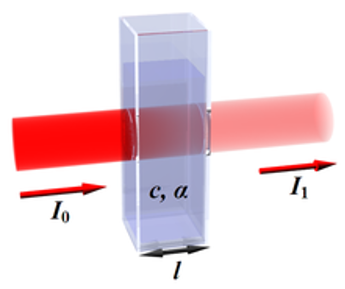
\includegraphics[width=.2\linewidth]{Ressources/Absorbance_cuve.png}

\end{document}
